\chapter{Results}
\index{Results@\emph{Results}}%

\section{Quantity Oppositions in Ictus position}


Ternary quantity contrast is only in primary stressed syllables. To analyze vowel duration measurements in all three quantities, a subset of only primary stressed syllables is taken from the dataset.
At the song level, the kalevala meter avoids short stressed syllables (Q1) in ictus position, preferring Q2 or Q3 (long and overlong) syllables to fall on the beat. In off-ictus postion, short stressed (Q1) syllables are preferred while Q3 avoided.


%\begin{figure}[htb]
%\centering
%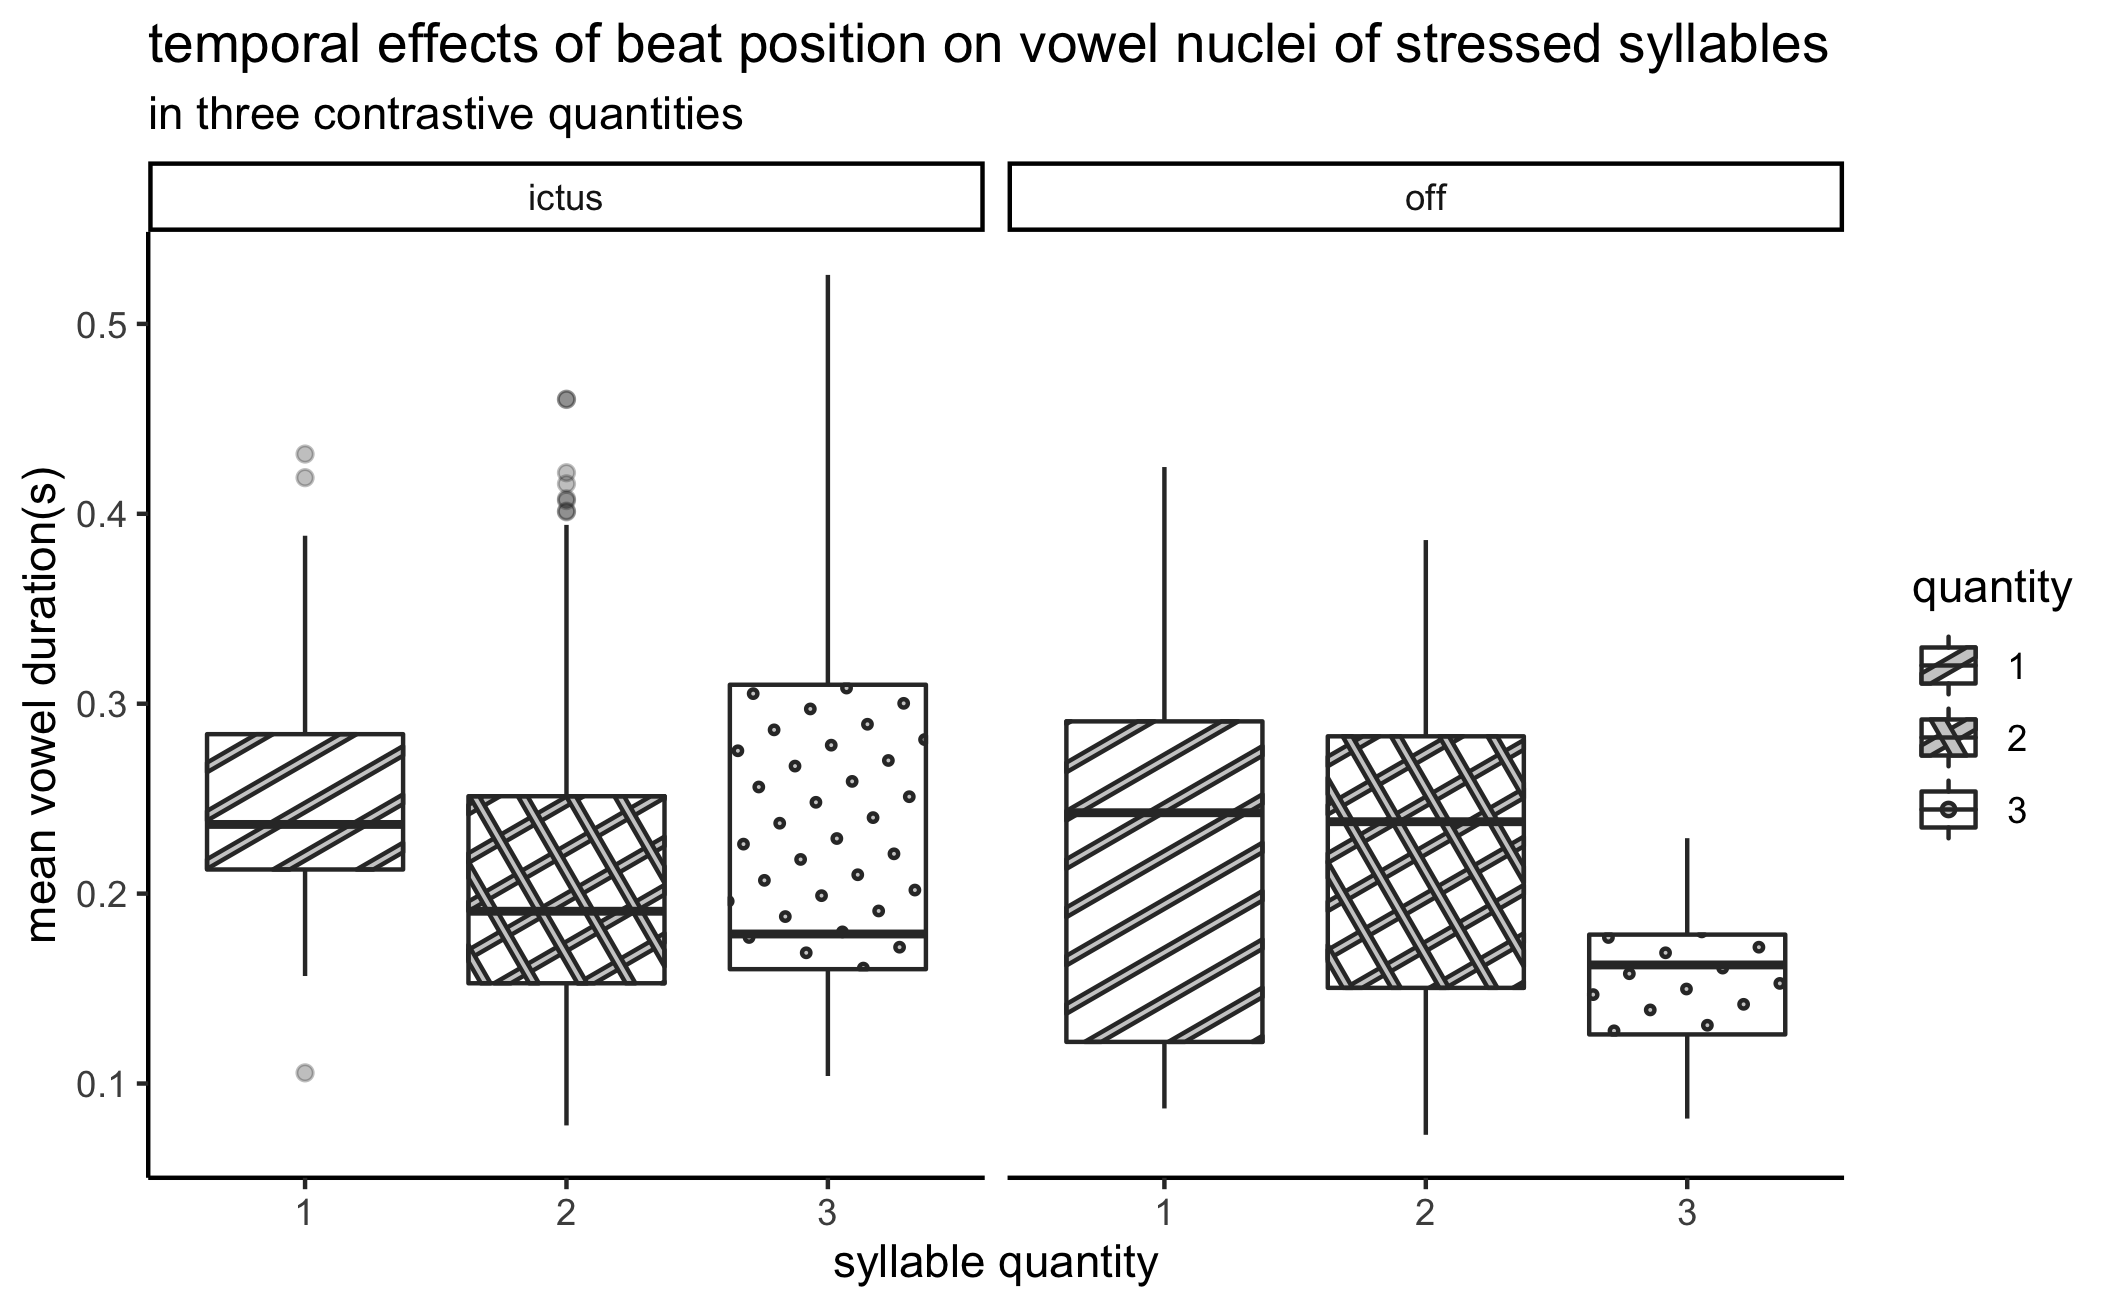
\includegraphics[width =\textwidth]{/Users/sarah/Git/regilaul_project/manuscript/results/q_dur.png}
%\caption{density plot of vowel durations in three syllable quantities}
%\label{qdur}
%
%\end{figure}
\begin{wrapfigure}{l}{0.5\textwidth}
\centering
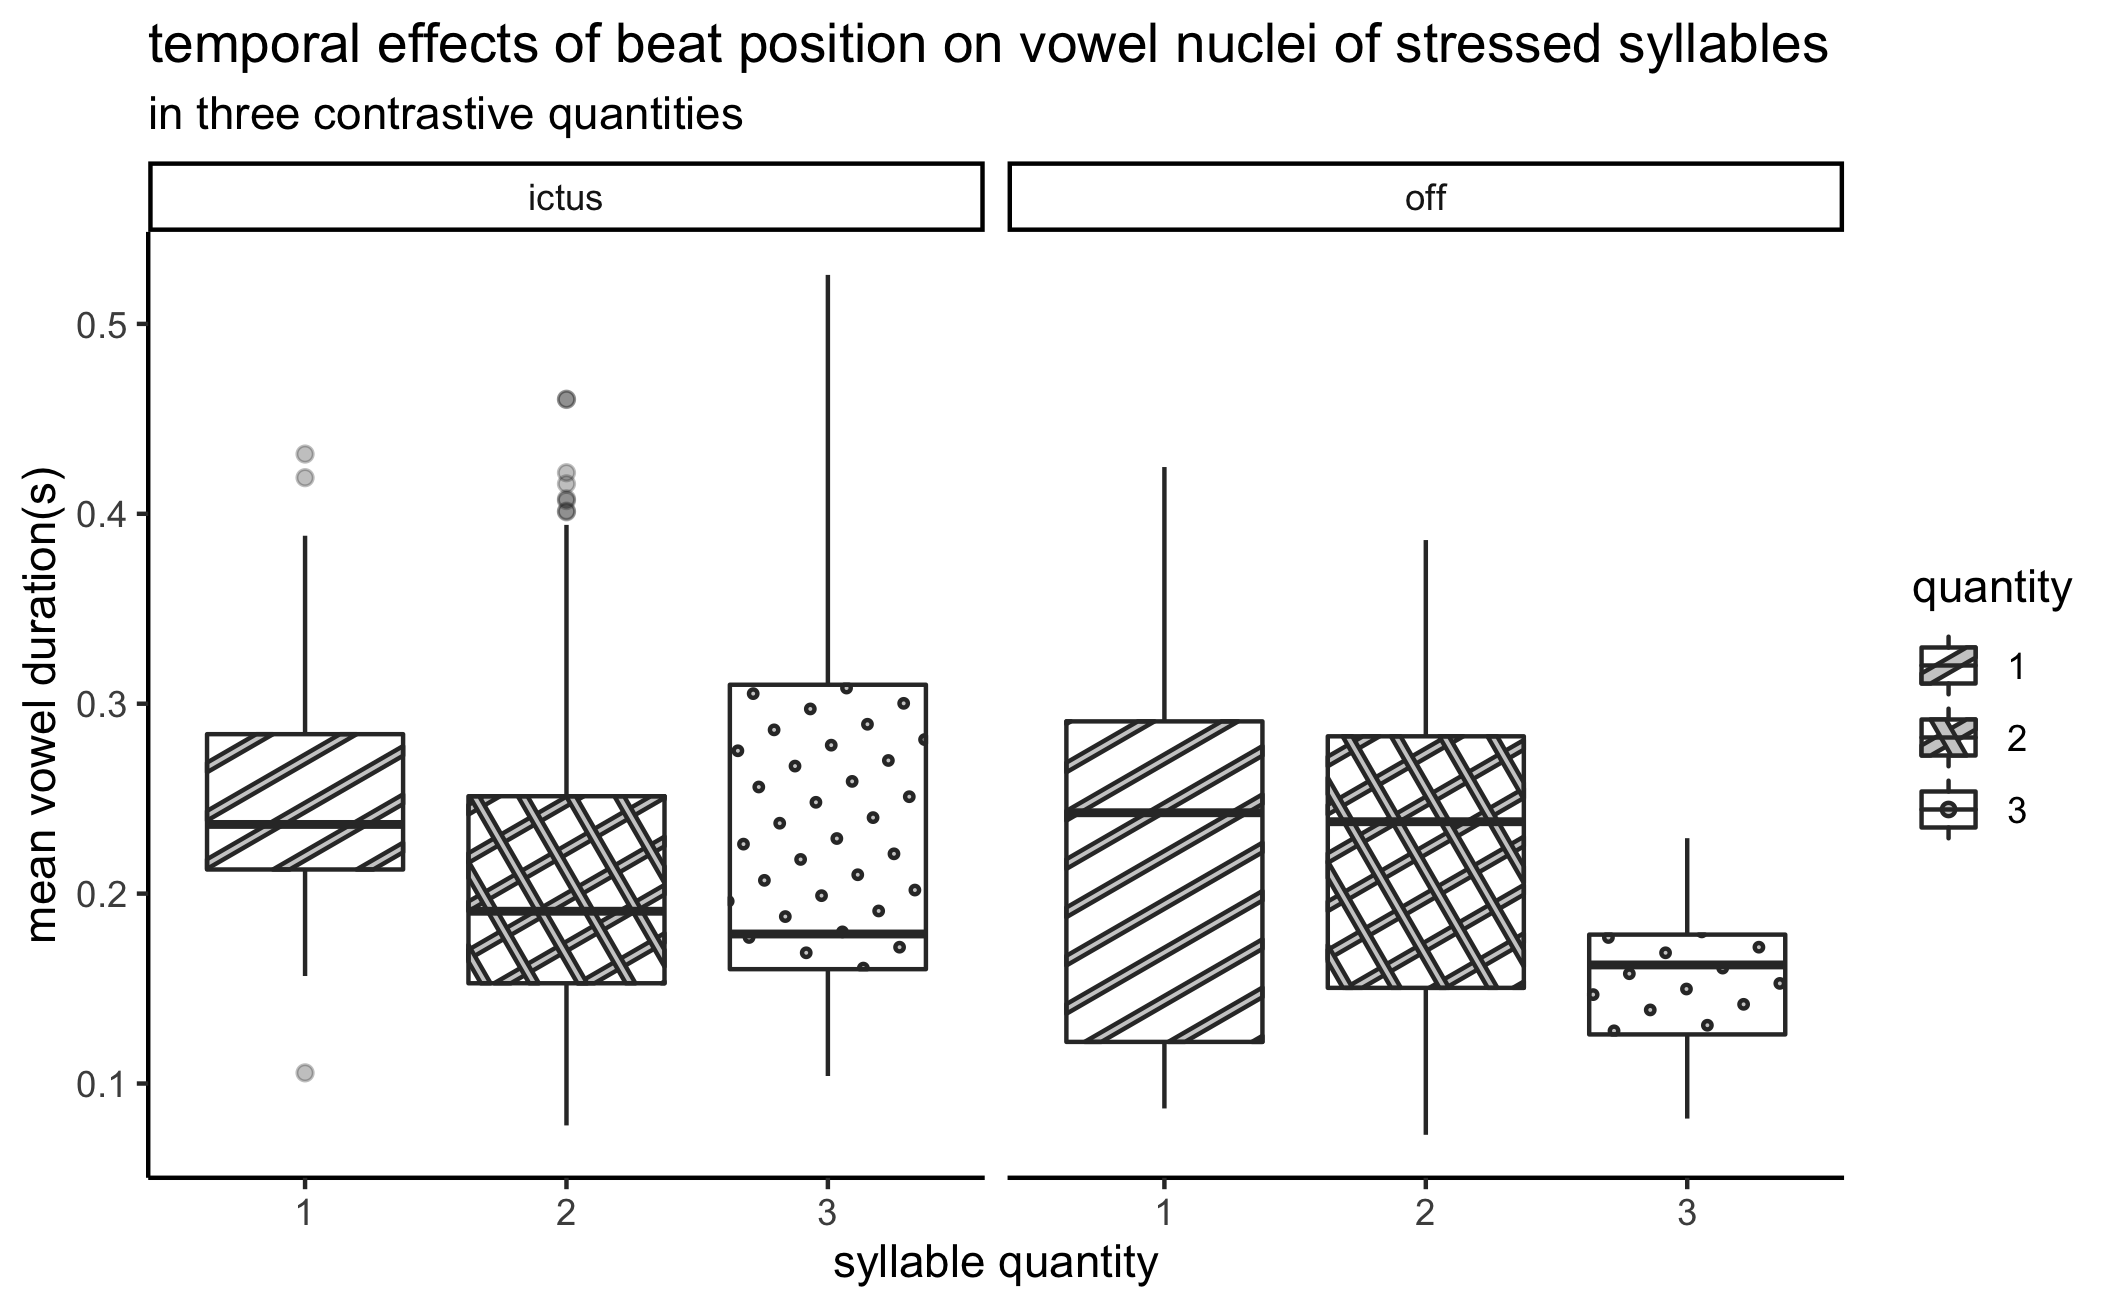
\includegraphics[width =0.5\textwidth]{/Users/sarah/Git/regilaul_project/manuscript/results/q_dur.png}
\caption{density plot of vowel durations in three syllable quantities}
\label{qdur}

\end{wrapfigure}


\ref{qdur} shows the vowel durations of all three syllable quantities, grouped by ictus and off-ictus positions in the song. In ictus position, median vowel duration descends as quantity increases, with the greatest difference between Q1 and Q2. Off the beat, a similar descending pattern is evident: however, in this case the largest difference is between Q2 and Q3 syllables. 
 The intercept is set at ictus position, Q1. Findings are significant results for Q2(p<0.001), Q3, and off-ictus positions (p< 0.05). Comparison with null model was statistically significant (p<0.001)\footnote{See Appendix A} 
 
 




%\begin{equation}
%$$lmer(duration ~ quantity + ictus + quantity * ictus + (1 | song) + (1 | word) + (1 | performer))$$ \\
%
%$$lmer(duration ~ (1 | song) + (1 | word) + (1 | performer))$$
%
%
%
%\end{equation}
\section{stress and unstress}


\subsection{duration}

Linear mixed-effects model results are significant for off-ictus (p<0.05), stressed (p<0.001), and Q2. Anova comparison of the maximal design model with a null model is also statistically significant. I reject the null hypothesis: these results support both word-level stress and beat position in song (ictus) as predictors for vowel duration. 

\begin{wrapfigure}{L}{0.5\textwidth}
\centering
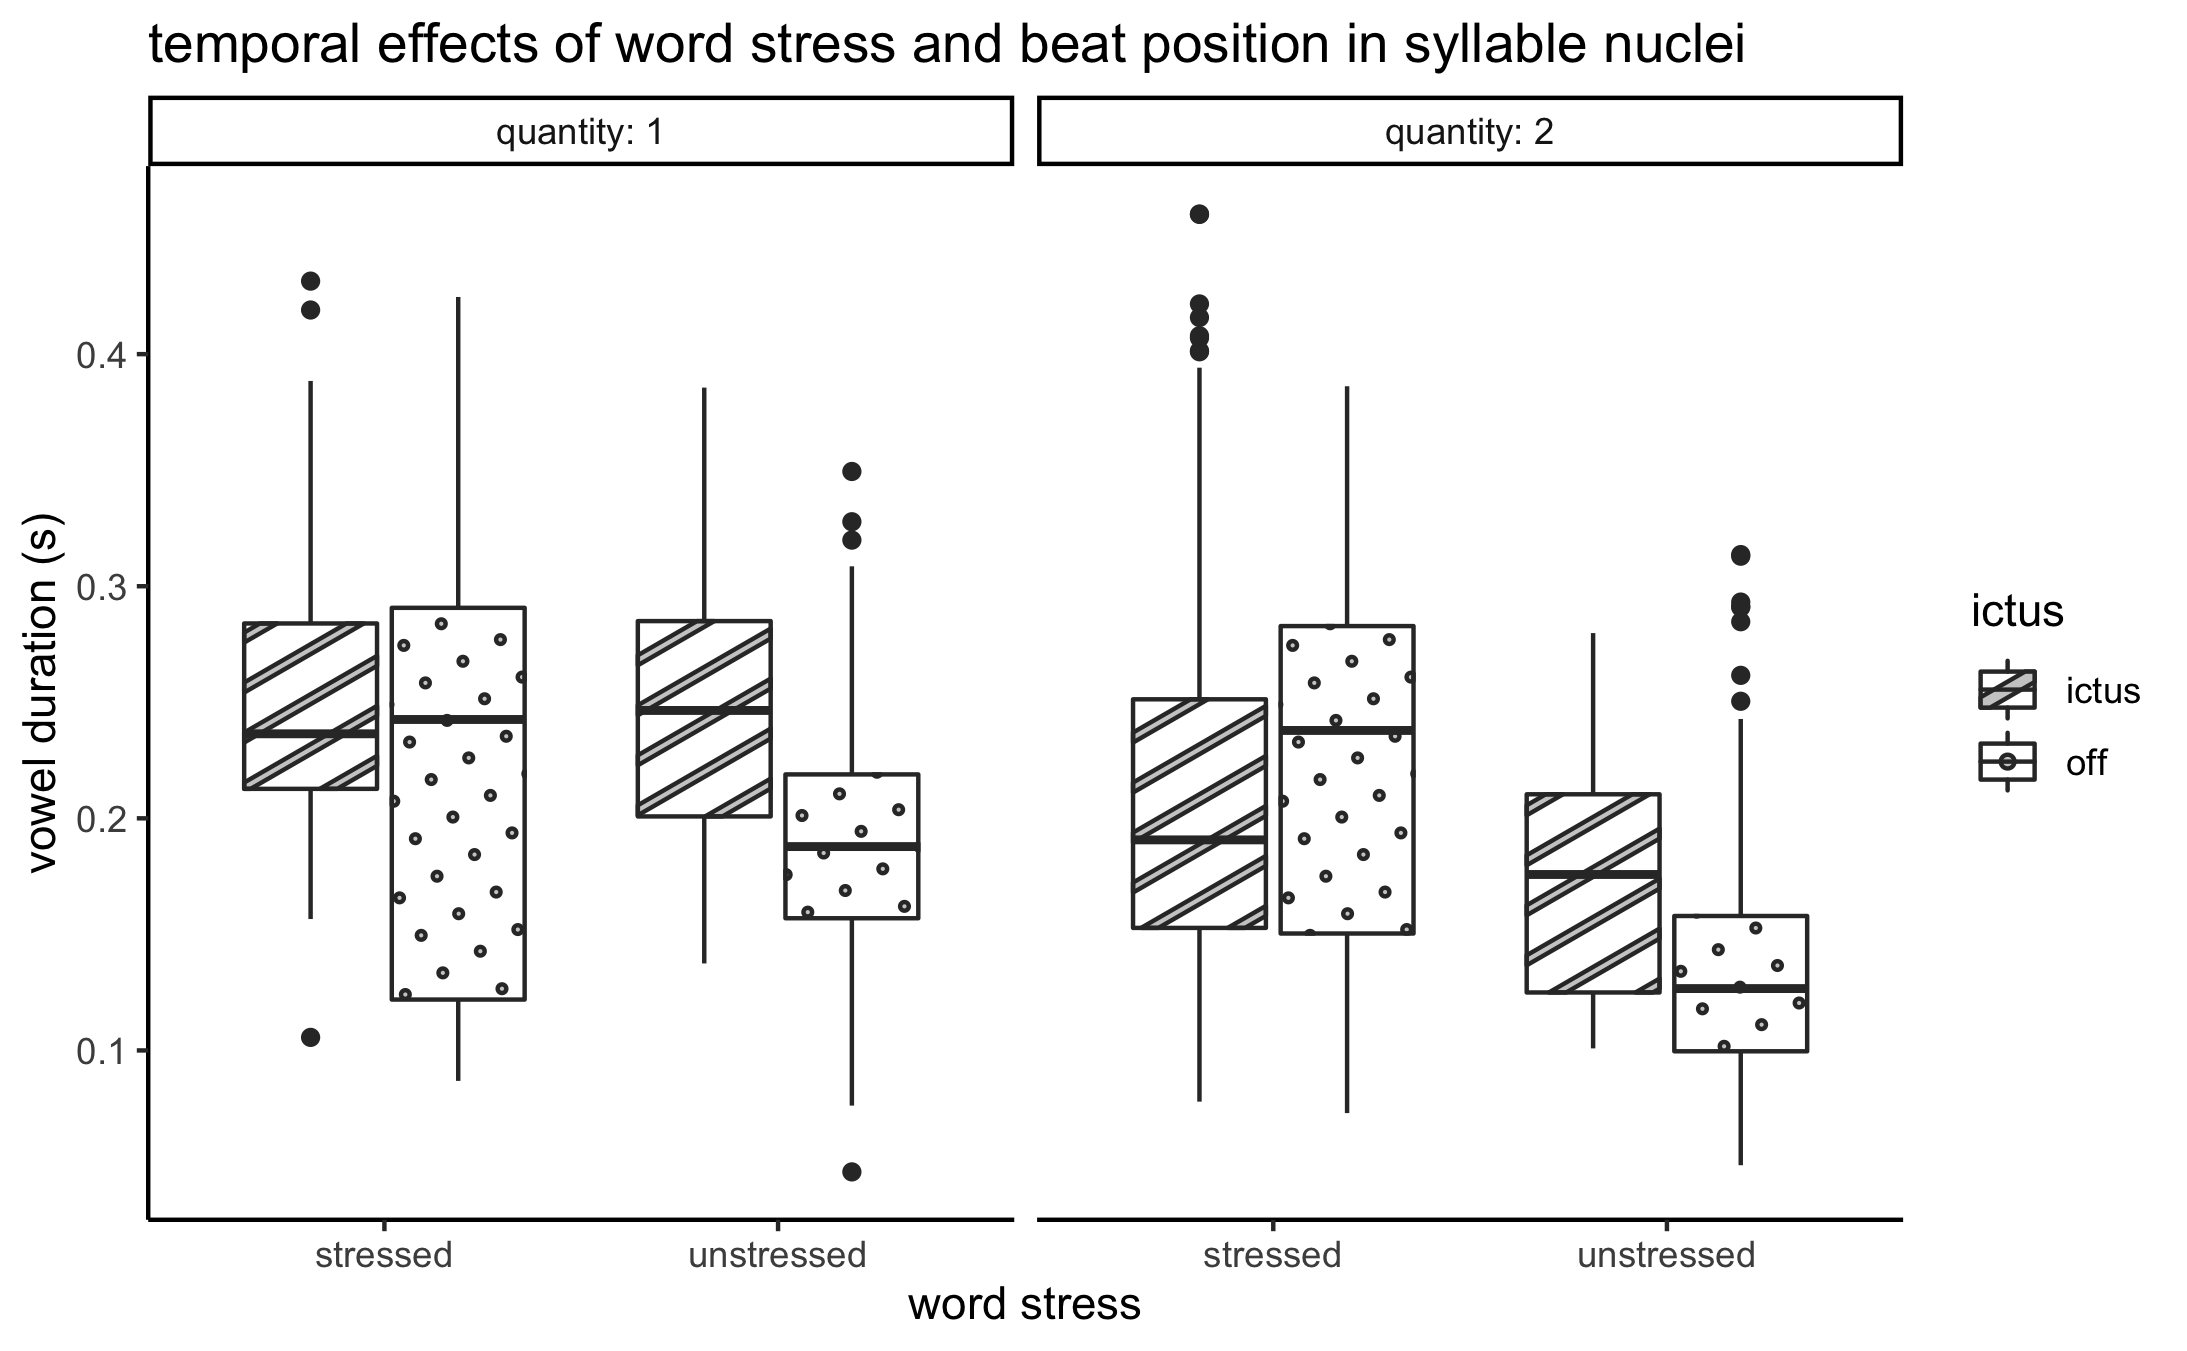
\includegraphics[width = 0.5\textwidth]{/Users/sarah/Git/regilaul_project/manuscript/results/dur_density_qfac.png}
\caption{vowel durations of stressed and unstressed Q1 and Q2 syllables falling on (ictus) and off the beat}
\label{durstrick}
\end{wrapfigure}
%%%%%%%%%%%%%%%%%%%%%%%%%%%%%%%%%%

\begin{wrapfigure}{R}{0.5\textwidth}
\centering
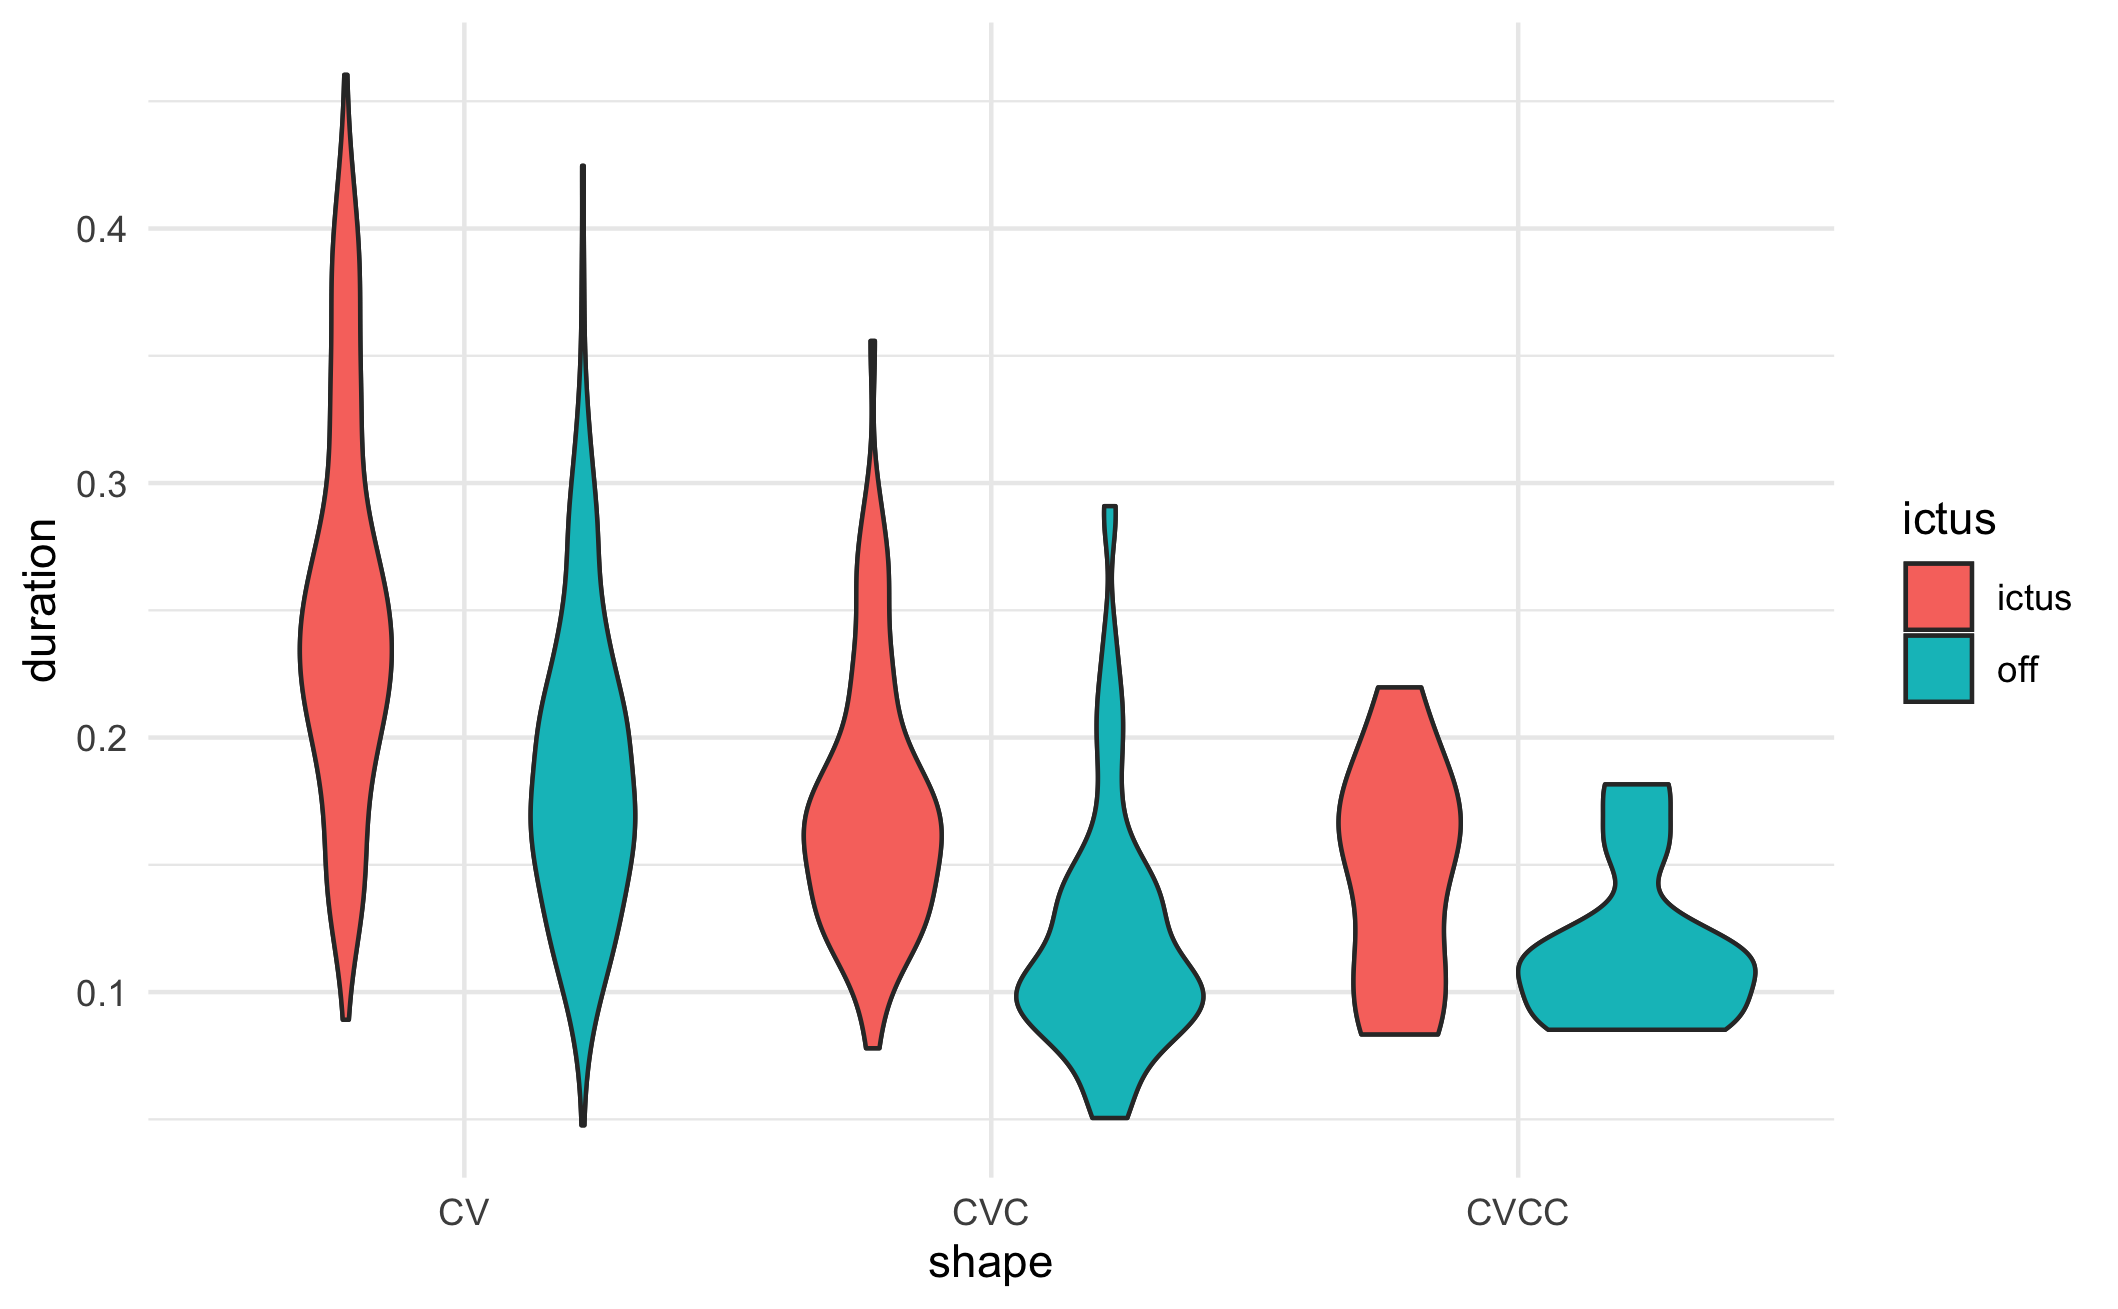
\includegraphics[width=0.5\textwidth]{/Users/sarah/Git/regilaul_project/manuscript/results/dur_shape_ictus.png}
\caption{vowel durations by beat position in open (CV), closed (CVC) and complex coda (CVCC) syllables}
\label{ickdursh}
\end{wrapfigure}

%%%%%%%%%%%%%%%%%%%%%%%%%%%%%%%%%%%%%%%%%%
\begin{wrapfigure}{L}{0.5\textwidth}
\centering
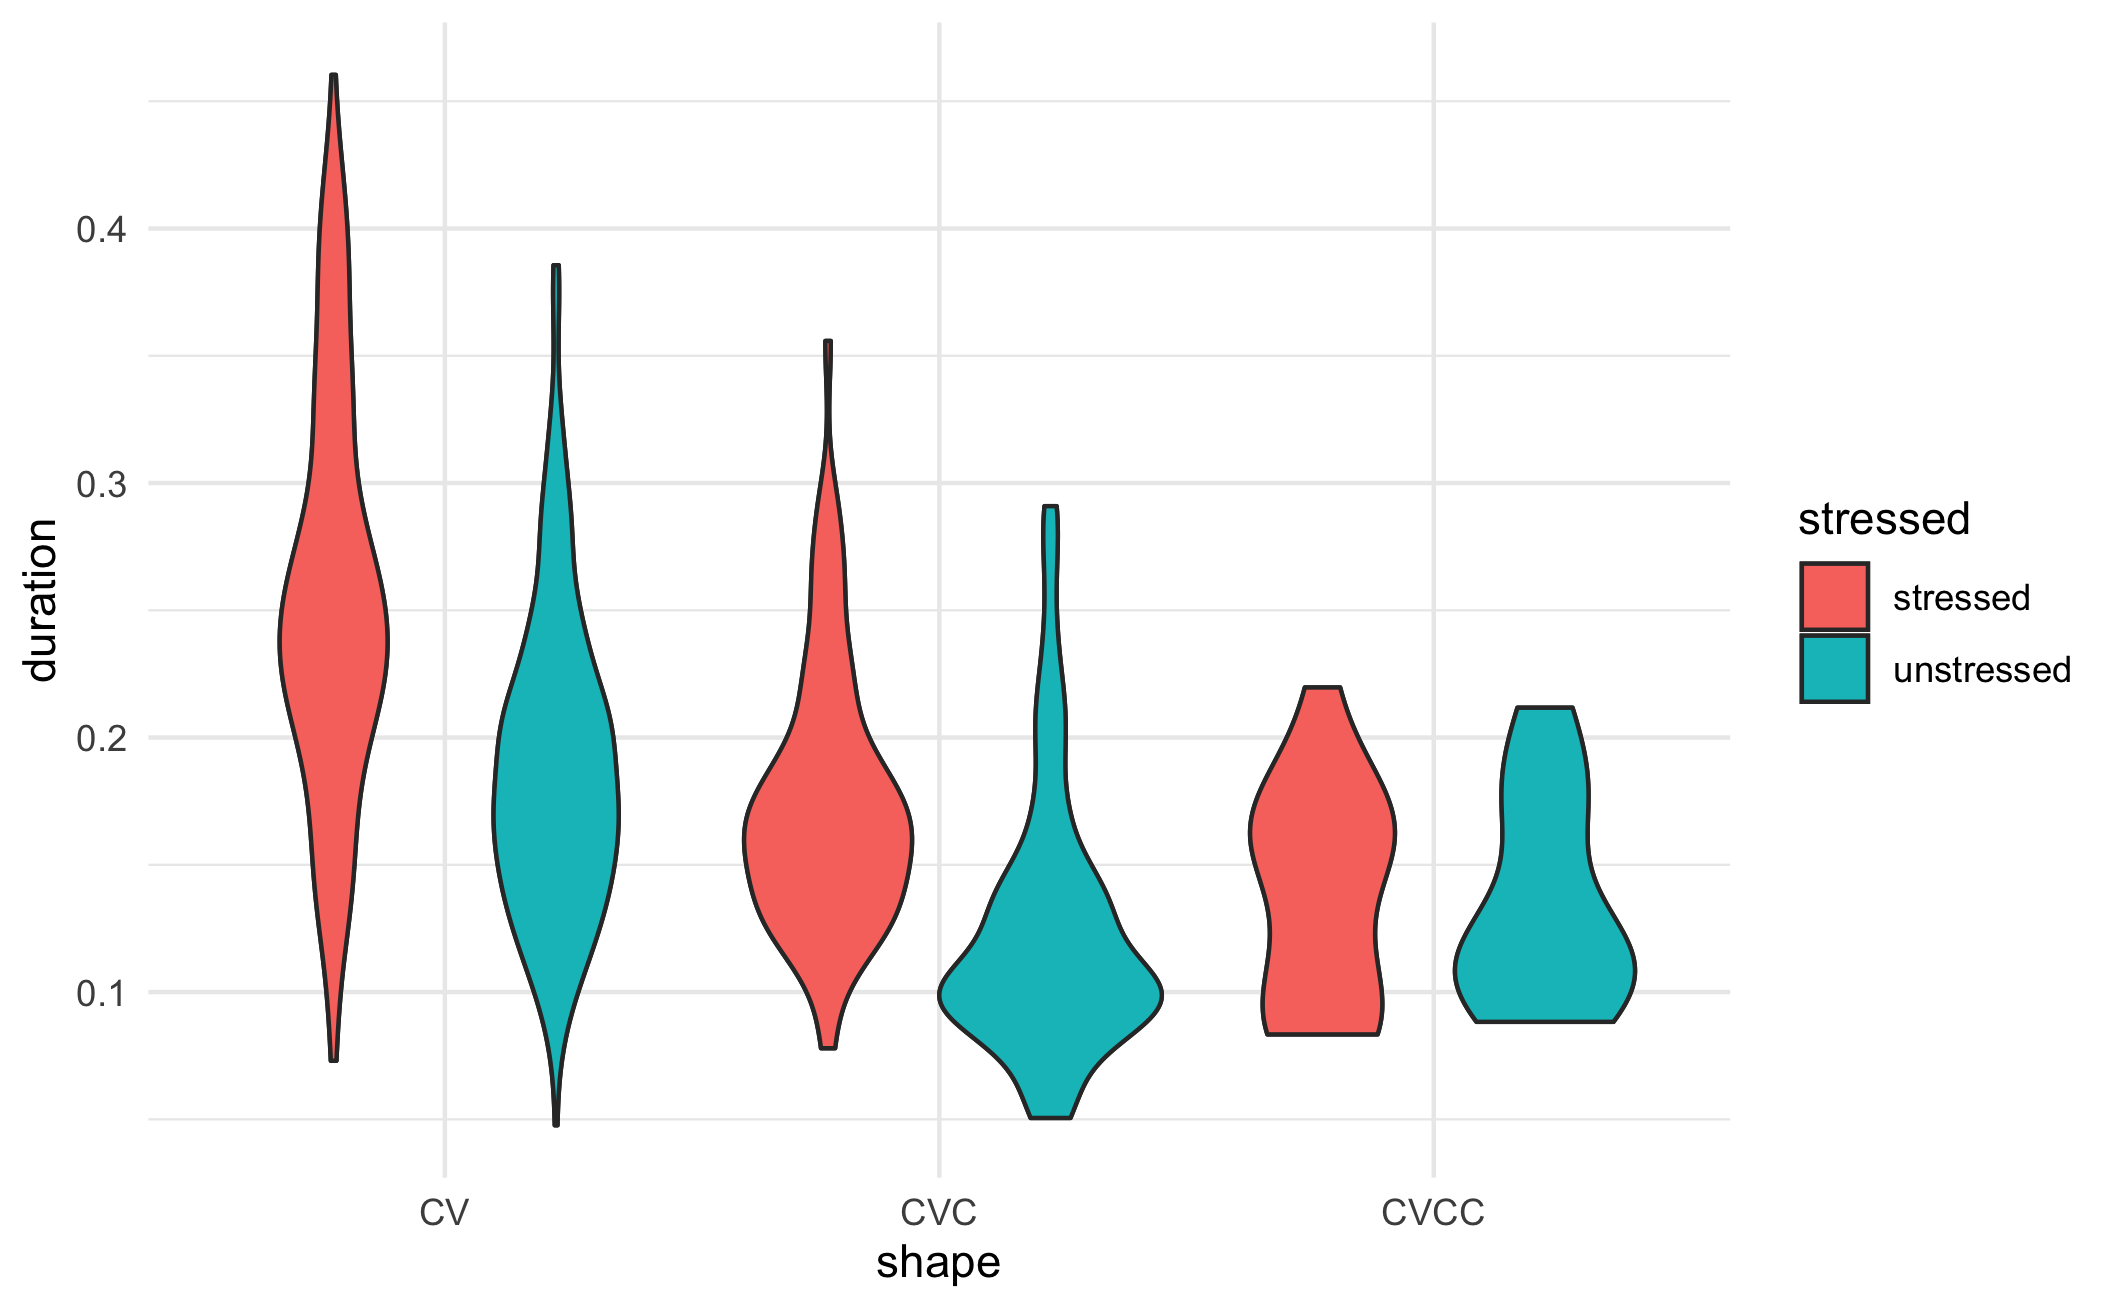
\includegraphics[width=0.5\textwidth]{/Users/sarah/Git/regilaul_project/manuscript/results/dur_shapestress.png}
\caption{vowel durations by word stress in open (CV), closed (CVC) and complex coda (CVCC) syllables}
\label{strdursh}

\end{wrapfigure}
%
%%%%%%%%%%%%

\subsection{space}

In vowel dispersion, only the intercept is significant. Comparison with null model is not statistically significant. Thus in the case of vowel dispersion, we fail to reject the null hypothesis. 
\begin{wrapfigure}{R}{0.5\textwidth}
\centering
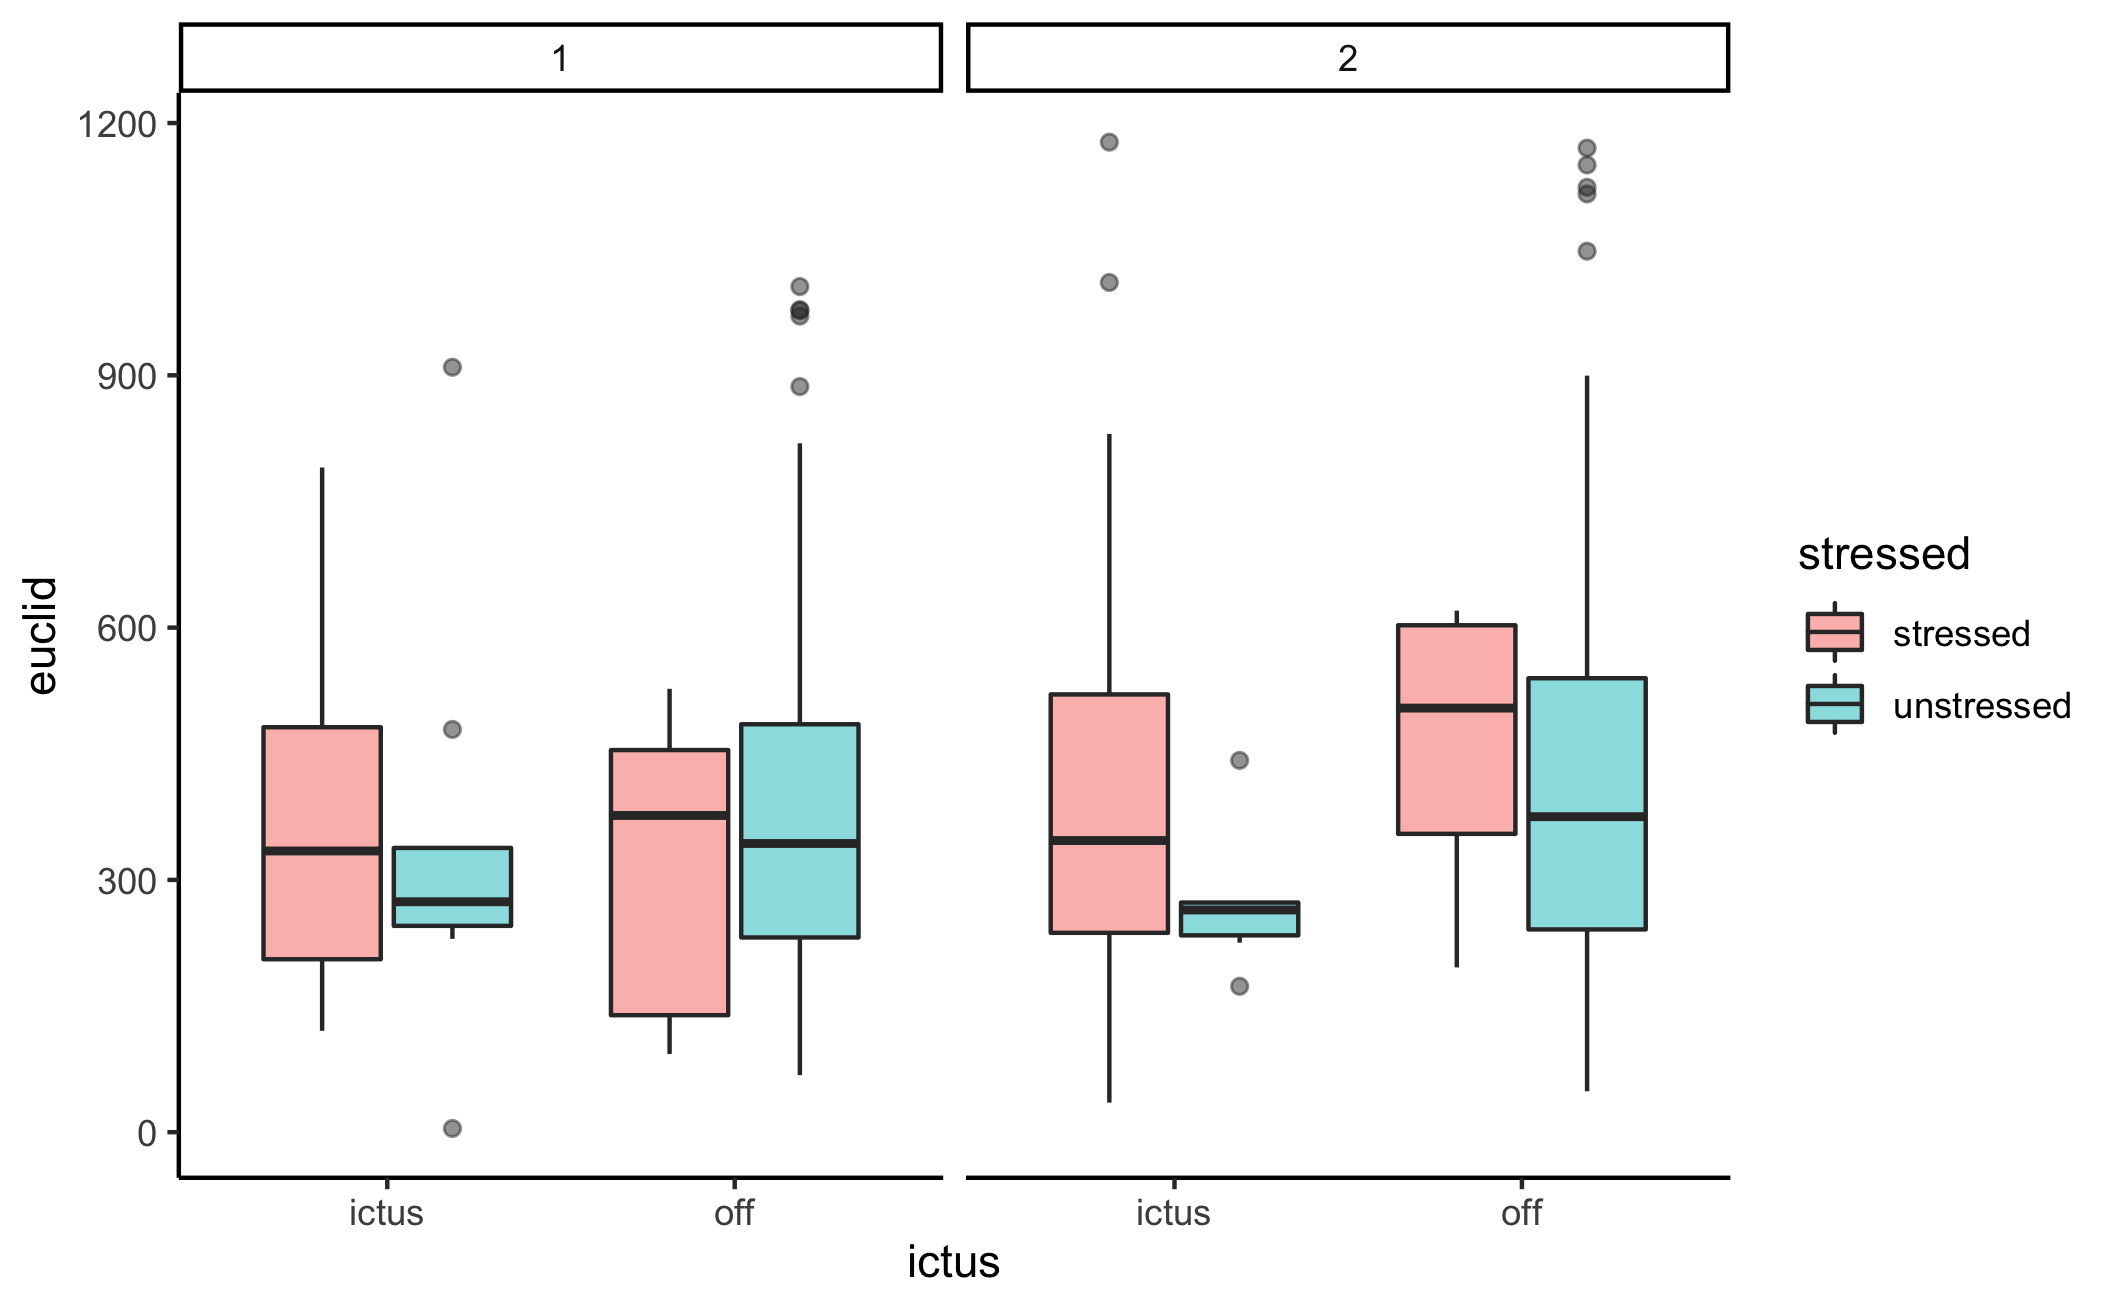
\includegraphics[width=0.5\textwidth]{/Users/sarah/Git/regilaul_project/manuscript/results/space_strictus.png}
\caption{euclidean distance of vowels in stress and ictus}
\label{spcstrick}

\end{wrapfigure}












